% \begin{frame}{Định nghĩa}
%     \begin{figure}[H] % places figure environment here   
%         \centering % Centers Graphic
%         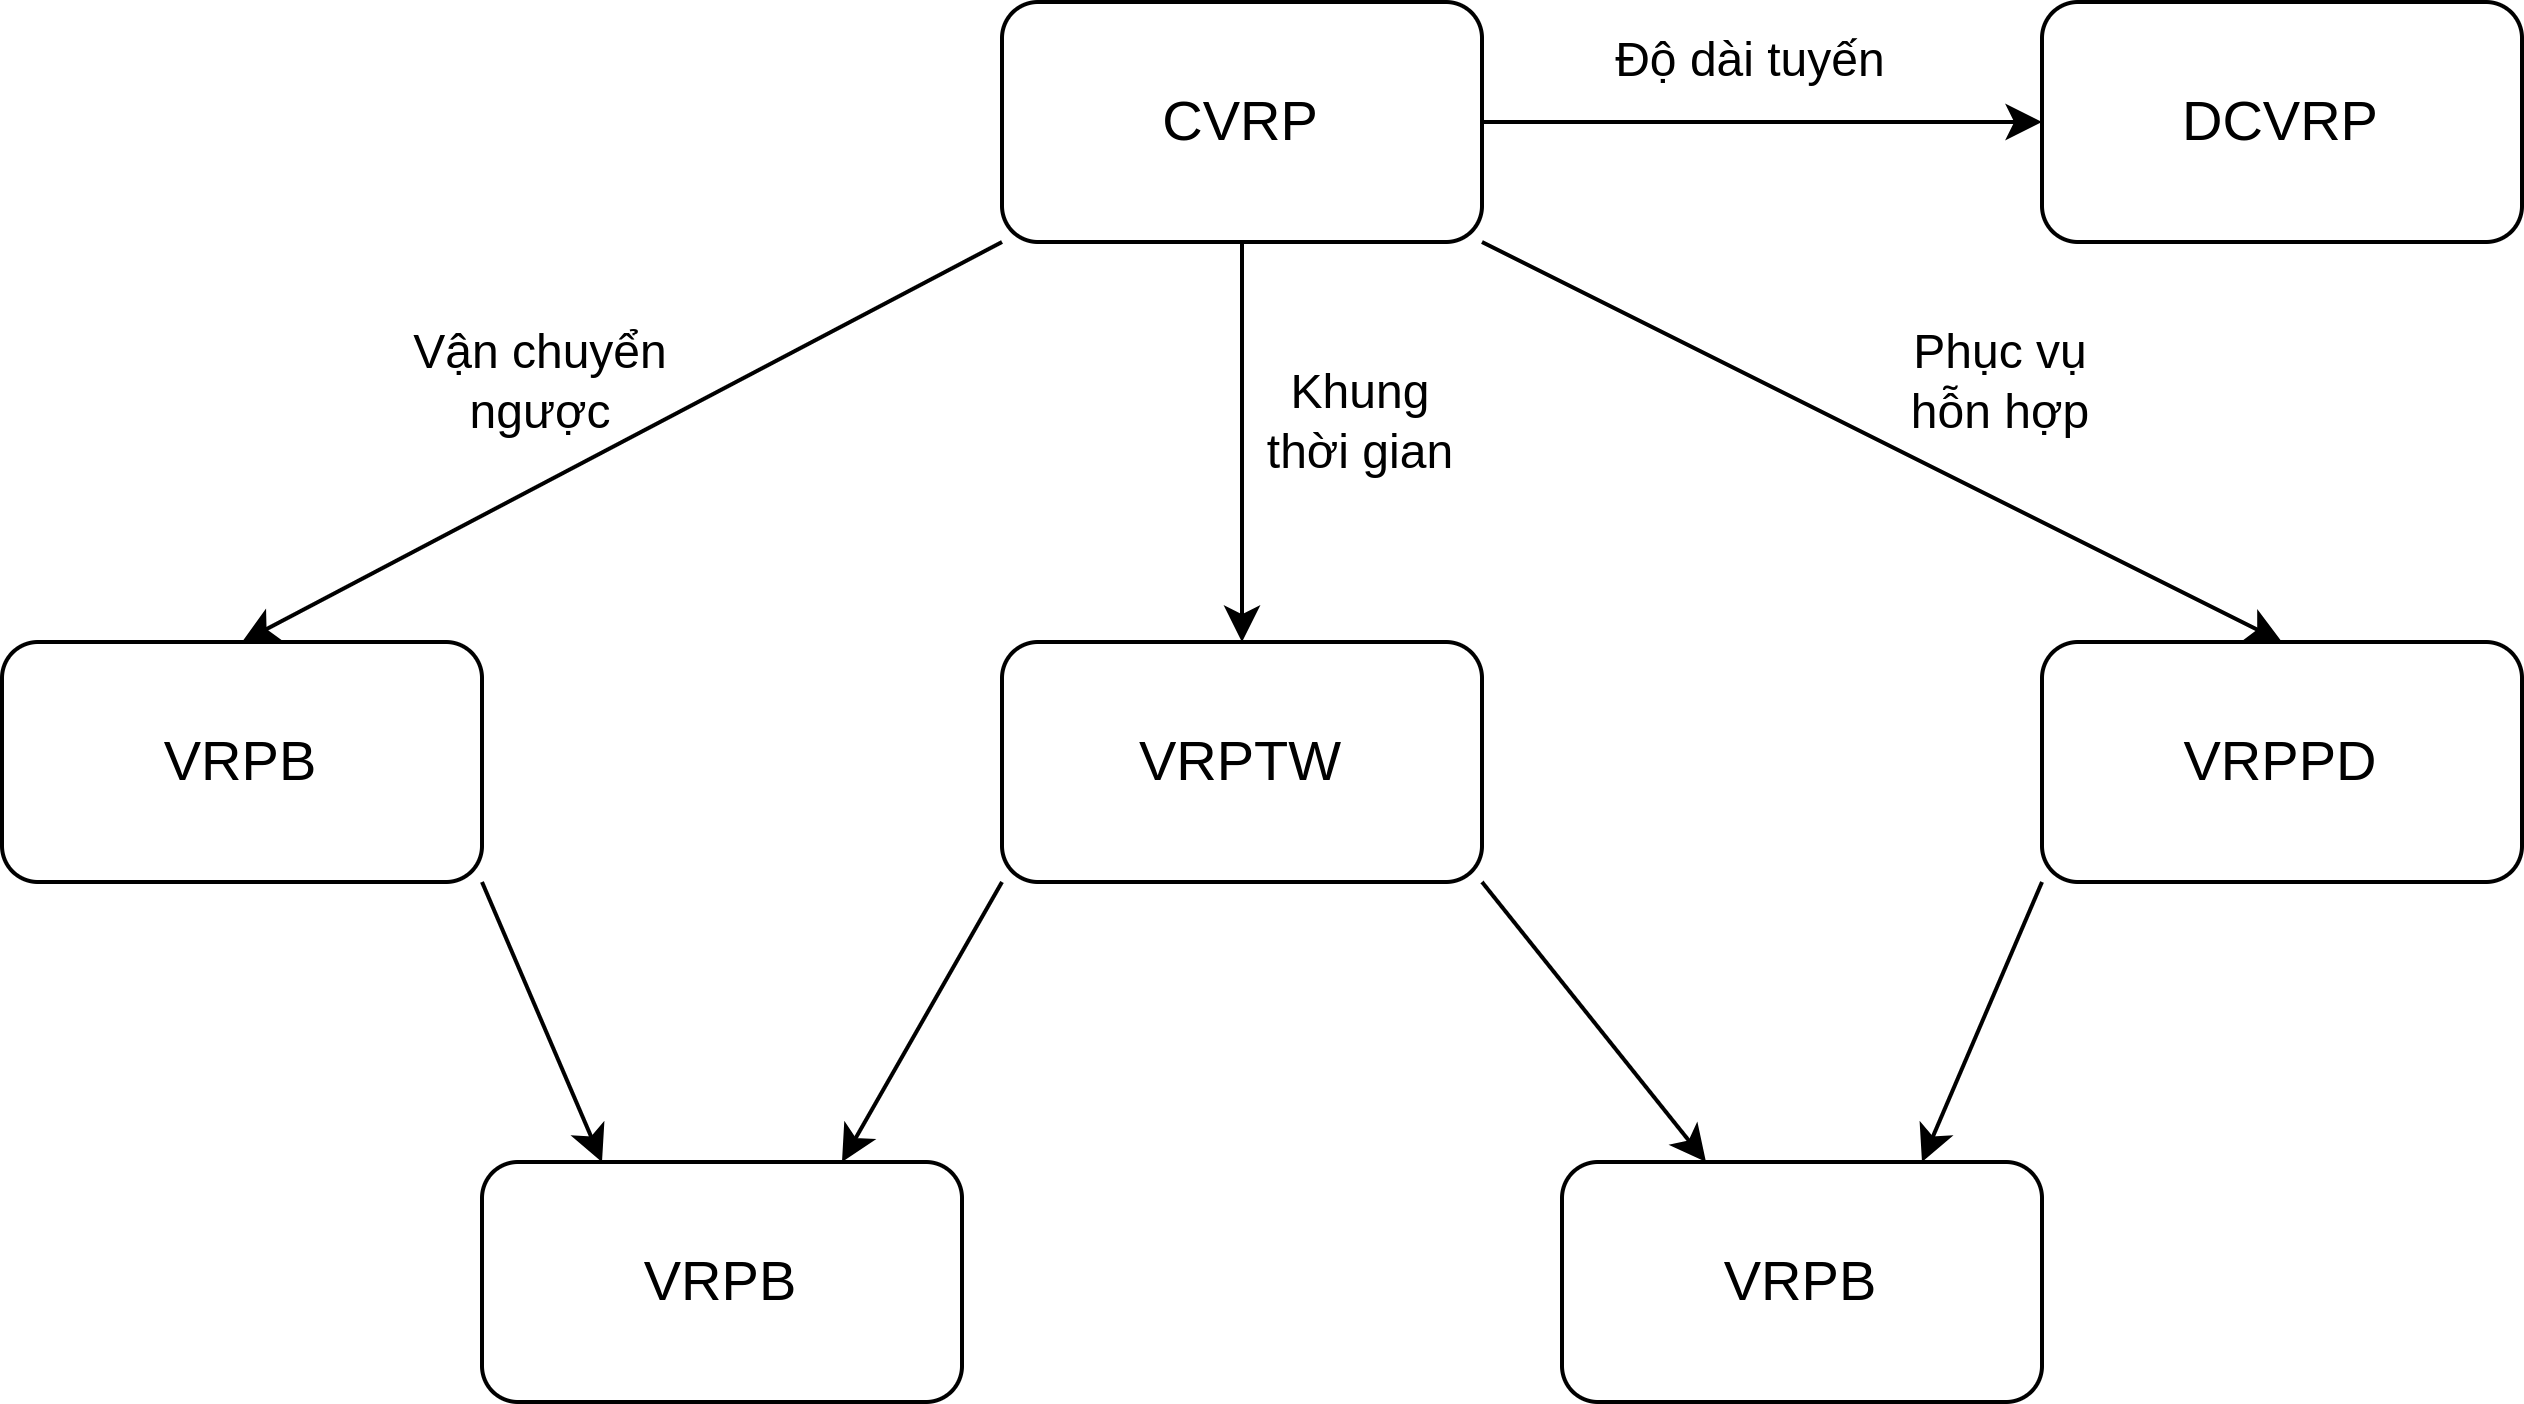
\includegraphics[width=0.8\textwidth]{figures/vrp.png} 
%         \caption{Các bài toán, biến thể của VRP} % Creates caption underneath graph
%         \label{fig:fg_01}
%       \end{figure}
% \end{frame}

% \begin{frame}{Định nghĩa}
%     \begin{block}{Định nghĩa theo ngôn ngữ lý thuyết đồ thị}
%         \begin{itemize}
%             \item Gọi $G=(V,A)$ là một độ thị đầy đủ với $V=\{ 0, ..., n \}$ là tập nút và $A$ là tập cung. Các nút $i=1,...,n$ đại diện cho các yêu cầu cần phục vụ, nút $0$ là kho hàng.
%             \item Một số không âm được gọi là chi phí $c_{ij}$ đại diện cho mỗi cung $(i,j) \in A$.
%             \item Bất đẳng thức tam giác cho chi phí
%             \begin{equation}
%                 c_{ij} + c_{jk} \geq c_{ik}, \quad \forall i,j,k \in V.
%             \end{equation}
%         \end{itemize}
%     \end{block}
% \end{frame}

% \begin{frame}{Định nghĩa}
%     \begin{block}{Định nghĩa theo ngôn ngữ lý thuyết đồ thị}
%         \begin{itemize}
%             \item Mỗi yêu cầu $i$ có một nhu cầu (về tải trọng) là $d_i$ và nhu cầu của kho $d_0=0$. Gọi $d(S) = \sum_{i \in S} d_i$ là tổng nhu cầu của tập.
%             \item Tập $K$ đại diện cho các xe, mỗi xe có tải trọng $C$, các xe ở kho tại thời điểm bắt đầu. Giả thiết $d_i \leq C$ với mỗi $i=1,...,n$.
%             \item $K_{min}$ là số xe ít nhất cần để phục vụ toàn bộ khách hàng.
%             \item Với một tập $S \subseteq V \setminus \{0\}$, gọi $r(S)$ là số xe ít nhất để phục vụ toàn bộ khách hàng thuộc tập $S$.
%         \end{itemize}
%     \end{block}
% \end{frame}

\begin{frame}{Định nghĩa - CVRP}
    Bài toán định tuyến xe với ràng buộc tải trọng (\textit{Capacited Vehicle Routing Problem - CVRP}) yêu cầu tìm một tập chính xác $K$ các chu trình (mỗi chu trình ứng với một tuyến đường) với tổng chi phí của tất cả các cung thuộc các chu trình này là nhỏ nhất. 
    \begin{block}{Các ràng buộc}
        \begin{itemize}
            \item[] (i) Mỗi chu trình đều đi qua nút ứng với kho hàng.
            \item[] (ii) Mỗi nút ứng với một khách hàng được đi qua bởi đúng một chu trình.
            \item[] (iii) Tổng nhu cầu của các khách hàng trong mỗi chu trình không được vượt quá tải trọng của xe.
        \end{itemize}
    \end{block}
\end{frame}

\begin{frame}{Định nghĩa - VRPTW}
    \begin{block}{VRPTW}
        \begin{itemize}
            \item Bài toán định tuyến xe với ràng buộc thời gian - VRPTW (\textit{VRP with time windows}) mở rộng CVRP. Mỗi khách hàng $i$ bị ràng buộc bởi một khoảng thời gian $[a_i, b_i]$ (\textit{time window}), thời gian phục vụ khách hàng $i$ là $s_i$.
            \item Nếu xe đến nút $i$ sớm thì phải chờ đến thời gian $a_i$ mới được phục vụ. Nếu xe đến nút $i$ muộn hơn $b_i$ thì khách hàng sẽ không được phục vụ.
        \end{itemize}
    \end{block}
\end{frame}

\begin{frame}{Định nghĩa - VRPTW}
    VRPTW yêu cầu tìm một tập chính xác $K$ chu trình với tổng chi phí là nhỏ nhất.
    \begin{block}{Các ràng buộc}
        \begin{itemize}
            \item[] (i) Mỗi chu trình đều đi qua nút ứng với kho hàng.
            \item[] (ii) Mỗi nút ứng với một khách hàng được đi qua bởi đúng một chu trình.
            \item[] (iii) Tổng nhu cầu của các khách hàng trong mỗi chu trình không được vượt quá tải trọng của xe.
            \item[] (iv) Với mỗi khách hàng $i$, thời gian bắt đầu phục vụ phải nằm trong khung thời gian $[a_i, b_i]$ và xe hoàn thành việc phục vụ sau khoảng thời gian $s_i$.
        \end{itemize}    
    \end{block}
\end{frame}

% \begin{frame}{Định nghĩa - kí hiệu}
    
% \end{frame}

% \begin{frame}{Mô hình - CVRP}
%     \textbf{Mô hình dựa trên dòng xe hai chỉ số }\\
%     $x_{ij}$ nhận giá trị bằng $1$ nếu cung $(i, j) \in A$ nằm trong nghiệm tối ưu và $0$ nếu trong trường hợp còn lại.
%     \begin{equation} \label{eq:vrp1}
%         \text{(VRP1)} \quad \min \sum_{i \in V} \sum_{j \in V} c_{ij} x_{ij}
%       \end{equation}
%       s.t.
%       \begin{flalign}
%           \label{ct_vrp1:1}  & \sum_{i \in V} x_{ij} = 1, \quad \forall j \in V \setminus \{0\}, \\
%         \label{ct_vrp1:2}  & \sum_{j \in V} x_{ij} = 1, \quad \forall i \in V \setminus \{0\}, \\
%         \label{ct_vrp1:3}  & \sum_{i \in V} x_{i0} = K,
%     \end{flalign}
% \end{frame}

% \begin{frame}{Mô hình - CVRP}
%     \begin{flalign}
%         \label{ct_vrp1:4}  & \sum_{j \in V} x_{0j} = K, \\
%         \label{ct_vrp1:5}  & \sum_{i \notin  S} \sum_{j \in S} x_{ij} \geq r(S), \quad \forall S \subseteq V \setminus \{0\}, S \neq \emptyset, \\
%         \label{ct_vrp1:6}  & x_{ij} \in \{0,1\}, \quad \forall i,j \in V.
%     \end{flalign}
% \end{frame}

% \begin{frame}{Mô hình - VRPTW}
%     \textbf{Mô hình dựa trên dòng xe ba chỉ số }\\
%     $x_{ijk}$ nhận giá trị 1 nếu xe $k$ đi trực tiếp từ nút $i$ tới nút $j$ và 0 nếu ngược lại.
%     \begin{equation} \label{eq1}
%         \min \sum_{k \in K} \sum_{(i,j) \in A} c_{ij} x_{ijk}
%     \end{equation}
%     s.t.
%     \begin{flalign}
%         \label{ct:1}  & \sum_{k \in K} \sum_{j \in \Delta^+(i)} x_{ijk} = 1, \quad \forall i \in N, \\
%         \label{ct:2}  & \sum_{j \in \Delta^+(0)} x_{0jk} = 1, \quad \forall k \in K,                   \\
%         \label{ct:3}  & \sum_{i \in \Delta^-(j)} x_{ijk} -  \sum_{i \in \Delta^+(j)} x_{jik} = 0, \quad \forall k \in K, j \in N,
%     \end{flalign}
% \end{frame}

% \begin{frame}
%     \begin{flalign}
%         \label{ct:4}  & \sum_{i \in \Delta^-(n+1)} x_{i,n+1,k} = 1, \quad \forall k \in K, \\
%         \label{ct:5}  & x_{ijk} (w_{ik} + s_i + t_{ij} - w_{jk}) \leq 0, \quad \forall k \in K, (i,j) \in A, \\
%         \label{ct:6}  & a_i \sum_{j \in \Delta^+(i)} x_{ijk} \leq w_{ik} \leq b_i \sum_{j \in \Delta^+(i)} x_{ijk}, \quad \forall k \in K, i \in N, \\
%         \label{ct:7}  & E \leq w_{ik} \leq L, \quad \forall k \in K, i \in \{0, n+1\}, \\
%         \label{ct:8}  & \sum_{i \in N} d_i \sum_{j \in \Delta^+(i)} x_{ijk} \leq C, \quad \forall k \in K, \\
%         \label{ct:9}  & x_{ijk} \geq 0, \quad \forall k \in K, (i,j) \in A, \\
%         \label{ct:10} & x_{ijk} \in \{0,1\}, \quad \forall k \in K, (i,j) \in A.
%     \end{flalign}
% \end{frame}